\begin{figure*}
    \centering
    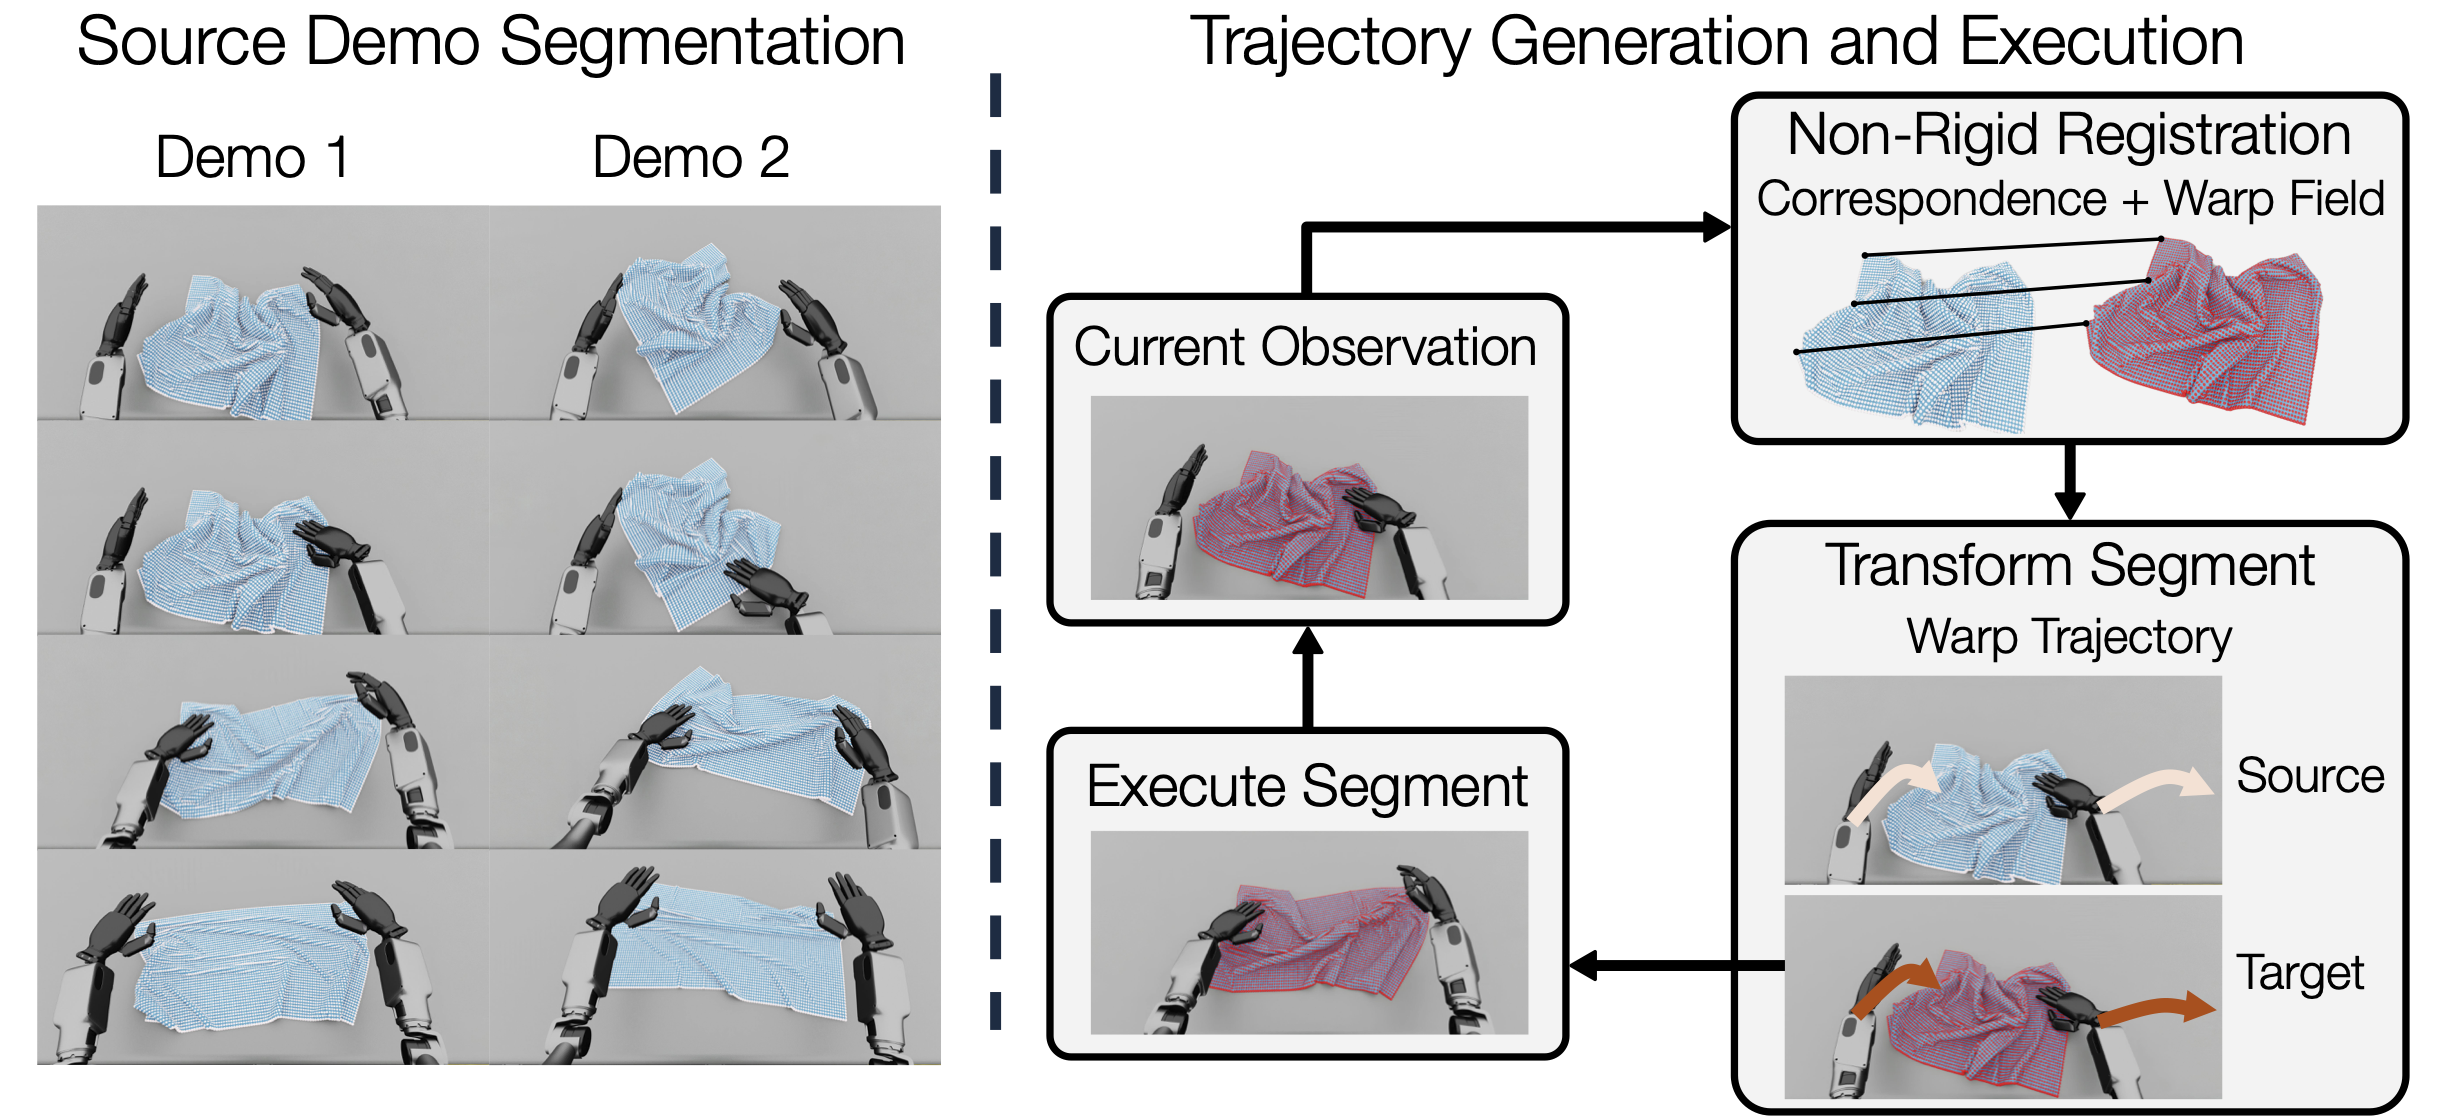
\includegraphics[width=0.82\textwidth]{Fig/Fig/Fig2.png}
    \caption{\textbf{\sysName\ System Pipeline.}
    \textit{(Left)} Human-teleoperated demonstrations are segmented into object-centric subtasks using manual annotations or heuristic signals, forming a library of source segments.
    \textit{(Right)} Given a new target scene, \sysName\ \textit{(i)}~observes the current deformable state, \textit{(ii)}~performs non-rigid registration to establish correspondence and a warp field between the source and target geometries (\textit{correspondence + warp field}), \textit{(iii)}~selects the source segment with the lowest registration cost and applies the resulting warp field to the end-effector trajectory (\textit{warp trajectory; source end-effector trajectory in light arrows, warped trajectory in darker arrows}), and \textit{(iv)}~executes the warped trajectory in the target environment.}
    \label{fig:fig2}
\end{figure*}